\chapter{Research of Previous Work}
\label{ch:previous}

A wooden seed-planting machine sits at an awkward intersection of three literatures that rarely cite one another. Precision-planter research measures singulation of maize, soybean and cotton on steel row units and treats the frame as rigid. Forestry and restoration research measures whether a hand jab, a hollow planting stick or a broadcaster puts a woody or native seed into a narrow depth band, and it treats the mechanism as a hand tool. Agricultural-robotics research plans coverage and tracks a path, and it treats the implement behind the hitch as a load rather than as a process whose quality collapses when the vehicle accelerates. This chapter reads those literatures in the order the two technologies of the thesis require. Section~\ref{sec:prev-meter} reviews metering, sensing and vision, which is the background of compliance-aware vision metering. Section~\ref{sec:prev-plan} reviews coverage and model-predictive tracking, which is the background of singulation-constrained terrain coverage. Section~\ref{sec:problem} turns the gaps into a problem set with indices, constraints and research questions. Throughout, a formula is quoted only when the later design uses it, and a numerical claim from the literature is kept attached to the paper that measured it.

\section{Research on vision-guided seed metering}
\label{sec:prev-meter}

\subsection{What the classical indices measure}

A precision meter is a device that tries to release one seed each time a cell, a finger or a vacuum orifice passes the drop gate. The agronomic object is not the gate. It is the spacing of plants after emergence, which nobody can see at the moment of release. The engineering substitute, standardised for single-seed drills, is the set of spacings measured on a greased belt or in a soil bin, classified against the target spacing \(x_{\mathrm{ref}}\) \cite{iso7256,kachman1995}. With the ordered spacings \(x_i\), the usual three classes are
\begin{equation}
\label{eq:classes}
\begin{aligned}
\text{multiple} &\quad\text{if}\quad x_i < 0.5\, x_{\mathrm{ref}},\\
\text{single} &\quad\text{if}\quad 0.5\, x_{\mathrm{ref}} \le x_i \le 1.5\, x_{\mathrm{ref}},\\
\text{miss} &\quad\text{if}\quad x_i > 1.5\, x_{\mathrm{ref}}.
\end{aligned}
\end{equation}
If \(N_{\mathrm{tot}}\) spacings are observed and \(N_s\), \(N_m\), \(N_u\) fall in the three classes, the quality-of-feed, miss and multiple indices are the frequencies
\begin{equation}
\label{eq:qfi}
\qfi = \frac{N_s}{N_{\mathrm{tot}}},\qquad
\mis = \frac{N_m}{N_{\mathrm{tot}}},\qquad
\mul = \frac{N_u}{N_{\mathrm{tot}}},\qquad
\qfi + \mis + \mul = 1.
\end{equation}
Kachman and Smith showed that a single coefficient of variation, taken over every spacing including the misses, confuses a meter that occasionally skips with a meter that scatters every seed \cite{kachman1995}. The precision index they recommend is the coefficient of variation inside the single class only,
\begin{equation}
\label{eq:cv}
\mathrm{CV}_s = \frac{1}{\bar{x}_s}\sqrt{\frac{1}{N_s-1}\sum_{i\in\mathcal{S}}(x_i-\bar{x}_s)^2},
\end{equation}
where \(\mathcal{S}\) is the set of singles. A meter can therefore be excellent on \(\qfi\) and still place singles with a scatter that a woody seedling, whose emergence window is a few millimetres of depth and a few centimetres of in-row position, will not forgive. Panning, Kocher, Smith and Kachman later took the same indices from the laboratory belt into sugar-beet fields and showed that the ranking of planters was not identical in the two settings, because soil flow and bounce after release are invisible on a greased belt \cite{panning2000}. That distinction matters for a wooden machine: the belt test sees the meter, and the furrow sees the meter plus the motion of the arm.

The kinematic relation that every later controller inverts is the match between plate rate and ground speed. With \(N\) cells on the plate and plate speed \(\omega\) in radians per second,
\begin{equation}
\label{eq:rate}
x_{\mathrm{ref}} = \frac{2\pi v}{N\omega}
\qquad\text{so}\qquad
\omega^{\star}(v) = \frac{2\pi v}{N x_{\mathrm{ref}}}.
\end{equation}
Equation~\eqref{eq:rate} is exact only when every cell releases exactly one seed, the release angle is constant, and the horizontal velocity of the seed relative to the soil is cancelled by the rearward component of the tube or by a brush. None of those conditions holds for a flattened, winged or irregular woody seed. Equation~\eqref{eq:rate} is still the feedforward term. Everything a vision loop adds is a correction around it.

\begin{figure}[ht]
\centering
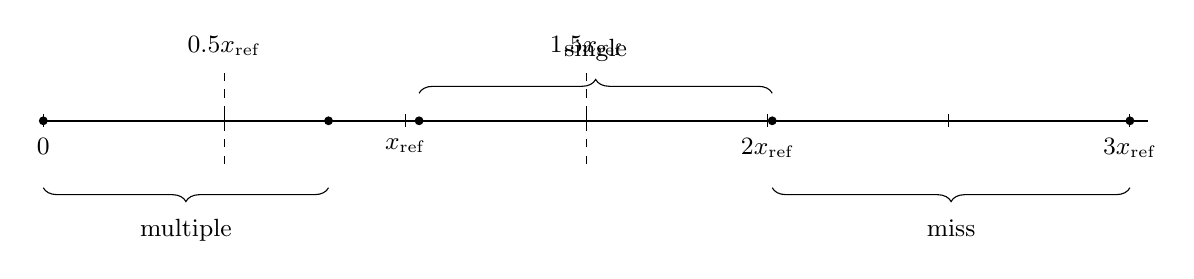
\begin{tikzpicture}[x=1.15cm,y=1cm,font=\small]
  \draw[thick] (0,0) -- (12.2,0);
  \foreach \x in {0,2,4,6,8,10,12} \draw (\x,0.08) -- (\x,-0.08);
  \node[below] at (0,-0.1) {\(0\)};
  \node[below] at (4,-0.1) {\(x_{\mathrm{ref}}\)};
  \node[below] at (8,-0.1) {\(2x_{\mathrm{ref}}\)};
  \node[below] at (12,-0.1) {\(3x_{\mathrm{ref}}\)};
  \fill (0,0) circle (1.6pt);
  \fill (3.15,0) circle (1.6pt);
  \fill (4.15,0) circle (1.6pt);
  \fill (8.05,0) circle (1.6pt);
  \fill (12.0,0) circle (1.6pt);
  \draw[decorate,decoration={brace,amplitude=5pt,mirror}] (0,-0.85) -- (3.15,-0.85) node[midway,below=8pt] {multiple};
  \draw[decorate,decoration={brace,amplitude=5pt}] (4.15,0.35) -- (8.05,0.35) node[midway,above=8pt] {single};
  \draw[decorate,decoration={brace,amplitude=5pt,mirror}] (8.05,-0.85) -- (12.0,-0.85) node[midway,below=8pt] {miss};
  \draw[dashed] (2,-0.55) -- (2,0.7);
  \draw[dashed] (6,-0.55) -- (6,0.7);
  \node[above] at (2,0.7) {\(0.5x_{\mathrm{ref}}\)};
  \node[above] at (6,0.7) {\(1.5x_{\mathrm{ref}}\)};
\end{tikzpicture}
\caption{Classification of successive seed spacings. The dashed lines are the ISO-style boundaries at half and one-and-a-half times the target spacing. A double close to a nominal site and a skip at the next site are one multiple and one miss, not two noisy singles.}
\label{fig:classes}
\end{figure}

Heege's survey of precision farming treats seeding as one actuation among several that become spatial once the machine knows where it is \cite{heege2013}. Ehsani, Upadhyaya and Mattson had already shown that a real-time kinematic satellite fix can map the intended seed coordinate to centimetre level \cite{ehsani2004}. Mapping the command is not the same as mapping the seed. Griepentrog, N{\o}rremark, Nielsen and Blackmore separated those two maps for sugar beet and argued that a seed map is the right input to later mechanical weeding \cite{griepentrog2005}. The distinction is the one this thesis keeps: a coverage planner produces a command map of where seeds should fall, and a metering controller produces an estimate of where they did fall. Lowenberg-DeBoer and Erickson, reviewing adoption, note that variable-rate and section control spread faster than the agronomy that would justify every rate change \cite{lowenberg2019}. For woody seed the justification is harsher than for maize, because the seed itself is scarce and the replacement cost of a failed hill is a year of growth rather than a later side-dress.

\subsection{Wooden tools and the depth band of woody seed}

The machines that actually put woody and native seed into the ground are, in a large part of the world, still hand tools, and many of those tools are wood or are used as if they were a stick. A Missoula Technology and Development Center evaluation of four commercial single-seed planters---a standard jab planter, a seed stick, a standing tube planter and a transplanter---found that hollow-tube tools with a bit that opens at the bottom planted small tree seed at a set depth more reliably than tools that merely poked and hoped, and that durability of the bit and of the release latch was the practical failure \cite{usdaplanter}. The operator supplied the singulation by dropping one seed into the tube. That division of labour is honest about mechanism: wood and a simple latch can make a hole, and they cannot see a double.

A jab planter built and tested by final-year bioresources students for no-till conditions assembled the same functions---frame and handle, hopper, precision meter, delivery tube, ground opener---into one manual machine, and compared it with a hoe \cite{jab2010}. The meter is the part that decides the index in Equation~\eqref{eq:qfi}. The frame is the part that decides whether the tube is vertical when the seed leaves it. A mechatronic dibbler built for a radiata-pine nursery attacked a related defect at production scale. Poorly shaped holes were bending stems; about \num{22}\% of seedling rejection at that nursery was attributed to the hole rather than to the plant. A machine that cut vertical holes of a specified depth removed the stem bend and raised worker throughput by about \num{10}\% \cite{dibbler}. The lesson for a field planter is not the nursery mechanism. It is the separation between a geometric specification (vertical, depth within a band) and a human or a servo that tries to meet it.

Masarei, Guzzomi, Merritt and Erickson measured the emergence of soft spinifex and found the optimum at a covering of \SI{5}{mm}, a sharp fall by \SI{10}{mm}, and almost no emergence from \SI{30}{mm}, on the rocky profiles of mine waste \cite{masarei2019}. They also record the practitioner survey result that depth precision is one of the properties restoration seeding lacks, and that agricultural openers built for crop seed do not hold a band of a few millimetres once the surface is rough. Bond, Honig and Maze had given the allometric reason: larger seeds reach the surface from deeper burial, so a depth setting copied from maize is not a conservative default for a small woody or native seed \cite{bond1999}. St Jack, Hesterman and Guzzomi, metering sandalwood seed, showed that a species with an irregular and relatively large woody seed still needs a meter designed around that shape rather than a crop plate with the vacuum turned up \cite{stjack2013}. This thesis takes a mid-size woody seed as its design case, with a target depth of \SI{18}{mm} and an estimation band of \(\pm\SI{8}{mm}\). Those two numbers are design assumptions, chosen to sit between the maize band and the spinifex band. They are not a measured optimum for a named species.

Wood enters the problem as structure, not as a romantic material. The Wood Handbook collects the design values: modulus of elasticity parallel to grain for common structural softwoods is on the order of \SIrange{8}{13}{GPa}, density is about a third to a half of aluminium, and internal friction in cellular tissue produces damping ratios that steel does not match without an added damper \cite{woodhandbook}. A row-unit link built as a timber cantilever of length \(L\), second moment \(I\) and modulus \(E\) has the tip stiffness
\begin{equation}
\label{eq:cantilever}
k = \frac{3EI}{L^3},\qquad I = \frac{bh^3}{12}
\end{equation}
for a rectangular cross-section bent about the strong or the weak axis according to how \(h\) is chosen. The equivalent mass \(m_{\mathrm{eq}}\) at the boot then sets the undamped frequency
\begin{equation}
\label{eq:fn}
f_n = \frac{1}{2\pi}\sqrt{\frac{k}{m_{\mathrm{eq}}}}.
\end{equation}
A steel parallelogram is usually designed so that \(f_n\) sits far above the disturbance spectrum of the ground. A timber link sized for a person to lift, or for a small nursery workshop to laminate, does not have that luxury. Roughness of wavelength \(\lambda\) met at speed \(v\) arrives at frequency \(v/\lambda\). When that frequency approaches \(f_n\), the dynamic magnification of a viscously damped oscillator,
\begin{equation}
\label{eq:mag}
M(r) = \bigl[(1-r^2)^2 + (2\zeta r)^2\bigr]^{-1/2},\qquad r = \frac{v}{\lambda f_n},
\end{equation}
grows without any change in the meter. Previous planter papers do not put Equation~\eqref{eq:mag} next to Equation~\eqref{eq:qfi}. That omission is the first gap this thesis works on. Soil-tool force models of the kind reviewed by Godwin and O'Dogherty supply the load that drives the flexure: draft and vertical force depend on depth, speed and a soil strength parameter, and they are large enough, on a light wooden boot, to move the set depth by millimetres \cite{godwin2007}. A cone index measured with the standard penetrometer is the field number those models are usually fed \cite{asabe313}.

\begin{figure}[ht]
\centering
\begin{tikzpicture}[font=\small, >=Stealth, scale=0.96]
  \draw[thick, fill=brown!25] (0,0) rectangle (2.3,0.28);
  \node at (1.15,0.14) {timber chassis};
  \draw[thick] (0.4,0.28) -- (0.4,1.7);
  \draw[thick] (1.9,0.28) -- (1.9,1.7);
  \draw[thick, fill=brown!40] (0.15,1.7) rectangle (2.15,2.55);
  \node[align=center] at (1.15,2.15) {hopper\\and plate};
  \draw[thick] (1.15,1.7) -- (1.15,0.55);
  \draw[thick, fill=black!10] (0.95,0.55) rectangle (1.35,0.15);
  \node[right] at (1.4,0.35) {boot};
  \draw[dashed] (2.5,2.3) -- (4.1,2.3);
  \draw[->] (4.1,2.3) -- (4.1,0.35);
  \node[right, align=left] at (4.2,1.3) {drop \(H\)\\flight \(t_f\)};
  \draw[<->] (2.35,0.28) -- (2.35,1.7) node[midway,right] {\(L\)};
  \draw[->] (1.15,0.15) -- (1.15,-0.45) node[below] {\(F_{\mathrm{soil}}\)};
  \node[align=left, anchor=west] at (4.2,2.6) {camera looks\\at the plate};
  \draw[->] (4.2,2.45) -- (2.2,2.2);
\end{tikzpicture}
\caption{Schematic row unit. The hopper and the plate sit on a timber link of length \(L\). Soil force at the boot deflects the link. The seed falls a height \(H\) after release, so any horizontal velocity of the moving gate becomes a spacing error.}
\label{fig:rowunit}
\end{figure}

\subsection{Optoelectronics and high-speed imaging}

Before a camera was cheap enough to mount on a row unit, singulation was measured with a light plane across the seed tube. Kocher, Lan, Chen and Smith built an optoelectronic sensor that timed seeds as they crossed a beam and converted inter-arrival time into spacing at a known ground speed \cite{kocher1998}. The method is fast, it needs no training set, and it cannot tell a clod of soil or a chip of husk from a seed, nor can it see two seeds that cross the plane overlapping. It also sees the seed only after the release decision is over, so it is a monitor unless a later cell can still be advanced or retarded.

High-speed imaging removed that ambiguity on the test stand. Mangus and colleagues mounted a camera at \num{300} frames per second on a variable-rate electric-drive planter and combined the frames with the machine's own speed and seed-tube pulses \cite{mangus2017}. Across constant speeds from \SI{2.4}{km/h} to \SI{16.1}{km/h} the mean singulation was \num{98.45}\%. Doubles were rare (\num{0.03}\%) and triples were absent in that data. The errors that did appear were organised by the operating state: they nearly doubled when the machine accelerated or decelerated at \SI{4.8}{km/h} per second rather than at \SI{2.4}{km/h} per second, and they rose once the meter was asked for more than about \num{1250} seeds per minute. Vision counts and the commercial seed-tube sensor agreed within \(0.8\pm 0.2\) percentage points. The paper's design recommendation is the one a coverage controller should read as a constraint. There exists a seed-per-minute region in which the meter is good, and headland behaviour knocks the machine out of that region even when the steady-state plate calibration is perfect.

Zhao, Gao, Su, Xu and Huang combined a discrete-element simulation of a high-speed meter with a high-speed camera, which is the right pairing when the object is the trajectory inside the housing rather than only the spacing on the belt \cite{zhao2024hs}. Discrete-element work itself goes back to Cundall and Strack's contact law for discs and spheres \cite{cundall1979}. Lei and colleagues used it, with a bench test, on a centralised rapeseed meter, where the seeds interact in a stream rather than in a single cell \cite{lei2021}. For a woody seed the contact parameters---friction with a timber or polymer wall, restitution after a bounce off a wooden tube---are not the maize parameters those studies identify. The method transfers. The numbers do not.

Navid, Ebrahimian, Gassemzadeh and Mousavinia showed that a laboratory camera and a classical image-processing chain, without a learned detector, already recover spacing statistics from a side view of falling seeds \cite{navid2011}. Classical processing is attractive on a wooden machine because the computing budget may be a single board. It fails when the seed is the same colour as the wooden tube, when dust coats the window, or when two overlapping silhouettes must be counted as two objects. Those are ordinary conditions in a restoration planting, and they are why the later papers move to learned detectors.

\subsection{Detectors that name an empty cell and a double}

Borja, Amongo, Suministrado and Pabico closed the loop, rather than only measuring it \cite{borja2018,borja2021}. A camera looked at the seed plate of a pneumatic maize meter. A processor labelled each hole filled or empty. A stepper advanced the plate to replace an empty hole before the gate. On \num{780} hole readings the vision error was \num{0.2564}\%. At simulated \SI{2}{km/h} and \SI{4}{km/h} the missed-hill count fell, relative to the same meter with the vision path disabled, by roughly half at the lower speed and by about a fifth at \SI{4}{km/h}. At \SI{6}{km/h} the vision-assisted meter missed \emph{more} hills than the open-loop meter. The authors trace the reversal to the microcontroller: image latency and a drive that could not hold a steady delivery rate once the hole period became short. The identification was accurate. The actuation was late. A late correction is not a neutral failure. It inserts a seed into a neighbour's interval and manufactures both a multiple and a miss.

That result is the empirical centre of the first technology. Any proposal that adds vision to a planter has to state the inequality between the hole period and the sum of exposure, inference and mechanism delay. With the feedforward of Equation~\eqref{eq:rate}, the hole period is
\begin{equation}
\label{eq:period}
\Delta t = \frac{x_{\mathrm{ref}}}{v} = \frac{2\pi}{N\omega}.
\end{equation}
A correction computed from an image is useful when it is applied to a cell that has not yet reached the gate, which means the processing delay \(\tau_v\) and the actuator delay \(\tau_a\) must satisfy
\begin{equation}
\label{eq:latency}
\tau_v + \tau_a < \eta\, \Delta t
\end{equation}
for a margin \(\eta < 1\) that covers jitter. Borja's rig crossed Equation~\eqref{eq:latency} between \SI{4}{km/h} and \SI{6}{km/h}. Mangus's electric-drive meter, watched rather than corrected, still singulated well at far higher speed because the meter itself was mechanically capable and the camera was not in the control path \cite{mangus2017}. The two papers are consistent. Measurement at high speed is solved more easily than correction at high speed.

Learned detectors changed what a frame can be asked. Blaser, Porter, Fuhrer and Bourlai trained YOLOv10 on peanut vacuum-meter videos from a test stand and from a planter, with augmentation for light and camera angle, and report a mean average precision at IoU \(0.5\) of \num{99.4}\% and an error of \num{1.91}\% on the three-way count of singles, empties and doubles \cite{blaser2024,wang2024yolov10}. Zhao, Wu, Cheng, Gao, Liu, Lai and Li paired an improved YOLOv5s with a SiamRPN++ tracker on a high-speed maize meter. Precision and recall of detection were \num{98.5}\% and \num{99.2}\%. Tracking was weaker (success \num{63.3}\%, precision \num{71.2}\%). The quality-of-feed error against a high-speed camera stayed under \num{3.3}\% from \SI{10}{km/h} to \SI{18}{km/h} \cite{zhao2025yolo}. Zhao, Xi, Shi, Zhang, Qu and Zhang had already put an improved YOLOv5s on the on-line detection of seeding performance, which is the deployment this thesis needs, as distinct from a bench score \cite{zhaoJ2023}. Bustos-Gayt{\'a}n and colleagues used machine vision to separate the influence of meter components and operating parameters on uniformity, which is the diagnostic use of the same pictures: the image is not only a count, it is evidence about which knob to turn \cite{bustos2025}.

\begin{figure}[ht]
\centering
\begin{tikzpicture}[x=0.95cm,font=\small, >=Stealth]
  \draw[thick] (0,0) -- (12.5,0);
  \foreach \x/\lab in {0/expose, 1.6/infer, 3.4/decide, 5.2/move plate, 8.2/gate}{
    \draw (\x,0.12) -- (\x,-0.12);
  }
  \draw[line width=2pt, blue!70!black] (0,0.45) -- (1.5,0.45) node[midway, above] {\(\tau_{\mathrm{exp}}\)};
  \draw[line width=2pt, blue!70!black] (1.6,0.45) -- (3.3,0.45) node[midway, above] {\(\tau_{\mathrm{nn}}\)};
  \draw[line width=2pt, orange!80!black] (3.4,0.45) -- (5.1,0.45) node[midway, above] {logic};
  \draw[line width=2pt, red!70!black] (5.2,0.45) -- (8.0,0.45) node[midway, above] {\(\tau_a\)};
  \draw[dashed] (8.2,-0.7) -- (8.2,1.15);
  \node[below] at (8.2,-0.7) {cell at gate};
  \draw[<->] (0,-1.15) -- (8.2,-1.15) node[midway, below] {must finish inside \(\eta\Delta t\)};
  \node[anchor=west] at (8.6,0.7) {if \(\Delta t\) shrinks,};
  \node[anchor=west] at (8.6,0.25) {the red bar};
  \node[anchor=west] at (8.6,-0.2) {crosses the gate};
\end{tikzpicture}
\caption{Latency budget of a corrective vision loop. Detection can be accurate and still harmful if the actuator command arrives after the empty cell has passed the release gate.}
\label{fig:latency}
\end{figure}

The detector papers and the Borja papers do not yet form one design. The detector papers evaluate a recording. Borja evaluates a correction and finds a speed at which the correction changes sign. Neither paper writes the wooden arm into the observation model. A seed that left the cell on time and then struck a vibrating wooden tube looks, in a tube camera, like a late seed. A filter that treats every late crossing as an empty cell will advance the plate and create the double Borja already saw from latency alone.

\subsection{Vacuum, contact mechanics and design inversion}

The pneumatic meter remains the reference mechanism because its pickup force can be written down. Karayel, Barut and {\"O}zmerzi modelled the vacuum pressure required to hold a seed against gravity and inertia as a function of orifice area, seed mass and the speed of the plate \cite{karayel2004}. In schematic form the pressure difference that holds a seed of mass \(m_s\) and projected area \(A_o\) against a centrifugal acceleration \(r\omega^2\) is of the order
\begin{equation}
\label{eq:vacuum}
\Delta p \ge \frac{m_s}{A_o}\bigl(g + r\omega^2 + a_{\mathrm{vib}}\bigr),
\end{equation}
where \(a_{\mathrm{vib}}\) is the extra acceleration of a compliant mount. Published forms of the model differ in the coefficients on friction and on the angle of the orifice. The term this thesis needs is \(a_{\mathrm{vib}}\). On a rigid steel meter it is a small residual. On a timber flexure near resonance it is the same order as \(g\), and a vacuum that was sized on a rigid rig will drop seeds that the sizing calculation declared safe. Singh, Singh and Saraswat optimised orifice, vacuum and speed for cotton and showed the familiar ridge in the response surface: too little vacuum misses, too much vacuum doubles, and speed shrinks the ridge \cite{singh2005}. An irregular woody seed widens the uncertainty on \(m_s/A_o\) because no two seeds present the same face to the orifice. That is an argument for a vision check even when the mean vacuum is correct, and it is an argument against copying a maize orifice into a wooden hopper and expecting the cotton response surface to reappear.

Maleki and colleagues measured a multi-flight auger as a grain-drill meter and found that volumetric devices, which are forgiving of seed shape, do not produce the single-seed spacing of Equation~\eqref{eq:classes} \cite{maleki2006}. For a restoration mix of several woody species a volumetric flute is sometimes the honest mechanism. For a single high-value woody species, where the thesis's indices apply, a cell plate or a vacuum plate remains the mechanism that vision can correct cell by cell. Anantachar, Kumar and Guruswamy trained a neural network on an inclined-plate meter and inverted it to propose design and operating parameters \cite{anantachar2010}. Inversion of a surrogate is useful when the plate geometry is the decision. It does not see a new seed lot, a film of pitch on a woody seed, or a flexure that was not in the training rig. On-line vision is the measurement the surrogate cannot replace. The two are complementary: the network proposes a plate and a nominal vacuum, and the loop of Section~\ref{sec:tech1} trims them while the machine moves.

Flight after release converts a small timing error into a spacing error. Under constant vertical acceleration from rest relative to the tube,
\begin{equation}
\label{eq:flight}
H = v_{z0} t_f + \tfrac12 g t_f^2.
\end{equation}
If the seed is simply dropped, \(v_{z0}\approx 0\) and \(t_f=\sqrt{2H/g}\). A horizontal velocity \(v\) of the machine, plus a horizontal velocity \(\dot{y}_{\mathrm{arm}}\) of the gate caused by arm flexure, carries the seed
\begin{equation}
\label{eq:carry}
\Delta x = \bigl(v + \dot{y}_{\mathrm{arm}}\bigr)\, t_f
\end{equation}
before it reaches the furrow. At \(H=\SI{0.42}{m}\), \(t_f\approx\SI{0.29}{s}\). At \(v=\SI{1.6}{m/s}\) the machine travels about \SI{0.47}{m} during the flight, which is more than twice the \SI{0.20}{m} design spacing of the woody-seed case. The tube and the furrow closer must cancel the mean of that transport. They cannot cancel a zero-mean vibration that changes from seed to seed. Equation~\eqref{eq:carry} is why arm velocity belongs in the metering filter and not only in a structural side calculation.

\subsection{What this line of work does not close}

The metering literature now contains accurate indices, a vacuum model, a discrete-element method, optoelectronic monitors, high-speed confirmation that acceleration and seed rate organise the errors, and detectors that name empties and doubles at errors of a few percent. It also contains one clear negative result: a correct detector plus a slow processor makes singulation worse above a modest speed \cite{borja2021}. It does not contain a filter whose process model is the flexure of a timber row unit, and it does not contain a speed command that refuses the resonance of that flexure and the latency limit of Equation~\eqref{eq:latency}. Those two missing pieces are one technology, because the same state vector carries the cell label and the arm motion. Section~\ref{sec:tech1} builds that technology. It cannot, by itself, decide which way the machine should drive across a slope, or how hard it may accelerate into a headland. That decision is the subject of the next section.

\section{Research on coverage planning and model-predictive tracking}
\label{sec:prev-plan}

\subsection{Coverage as a geometric problem}

Coverage path planning asks for a path whose swept width paints a region and whose cost, usually length or time, is small. Choset's survey fixed the vocabulary: cellular decomposition, Morse functions, and the boustrophedon pattern in which the machine runs a straight swath, turns on a headland, and runs the next swath in the opposite direction \cite{choset2001}. Galceran and Carreras updated the survey across robotics and separated off-line planners, which assume a known map, from on-line planners, which discover the boundary as they travel \cite{galceran2013}. A seed-planting machine of the kind considered here is an off-line planner at the scale of the field and an on-line controller at the scale of the swath. The boundary is known from a survey or from a previous pass. The disturbance that matters is not an unknown wall. It is a grade, a patch of soft soil, and a meter that misbehaves when the speed profile is aggressive.

Oksanen and Visala published coverage algorithms aimed at agricultural field machines rather than at indoor robots, including the treatment of headlands, obstacles and the choice of driving direction on real field polygons \cite{oksanen2009}. LaValle's planning text supplies the underlying algorithms---grid search, sampling, feedback on a cell complex---that those field methods specialise \cite{lavalle2006}. Dijkstra's shortest paths and the A* search of Hart, Nilsson and Raphael remain the workhorses inside a grid once a field has been rasterised \cite{dijkstra1959,hart1968}. They are optimal on the grid they are given. They are silent on whether the cost of an edge should be metres, joules, or expected missed seeds. Putting the wrong scalar on the edge is not a small modelling choice. It is the difference between a short path and a path the meter can survive.

Bochtis and Vougioukas minimised the non-working distance of a machine that covers a field in a headland pattern, which is the distance spent turning and relocating rather than sowing \cite{bochtis2008}. Bochtis, S{\o}rensen and Busato reviewed the wider machinery-management problem: sequencing of fields, capacity of the machine, and the distinction between a path that is short and a plan that a fleet can execute \cite{bochtis2014}. S{\o}rensen and Bochtis had set out the fleet-management concepts that sit above a single planter \cite{sorensen2010}. Spekken and de Bruin optimised in-field routing by counting manoeuvring and servicing time, which is the right objective when the expensive event is the turn rather than the metre of straight work \cite{spekken2013}. Edwards and colleagues evaluated a prototype in-field route planner on neutral-material-flow operations and showed that a planner's predicted gain survives contact with a real sequence of loads only if the model of service time is honest \cite{edwards2017}. Fountas and colleagues place all of these plans in a farm management information system, which is where a seed map and a coverage file have to live if a later operation is to find them \cite{fountas2015}. This thesis stops at one machine and one field. The interface it leaves upward is a coverage file and a per-row seed estimate, which is what those information systems already know how to store.

\subsection{Driving direction, headlands and three-dimensional energy}

On flat ground the best driving direction is mostly a statement about how many turns fit along the short side of the field. Hameed, Bochtis, S{\o}rensen and N{\o}rremark generated guidance lines for operational planning and made the driving angle a decision variable rather than a habit of the operator \cite{hameed2010}. Jin and Tang solved coverage on two-dimensional field surfaces with an explicit cost on turns and on overlapped or missed area \cite{jin2010}, and then lifted the same problem onto three-dimensional terrain, where the slope changes the cost of each heading and can change the decomposition of the field \cite{jin2011}. The three-dimensional statement is the one a wooden planter on a restoration slope needs. A heading that is only a few degrees off the contour carries a sustained component of weight down the drawbar.

Vahdanjoo, Gislum and S{\o}rensen built a three-dimensional coverage tool for a seeding operation, using a digital elevation model to choose the driving direction against an energy criterion, and they also produced a variable-rate map and a compaction-risk estimate \cite{vahdanjoo2023}. On two sample fields their model reduced the required energy by up to \num{9.5}\% and \num{15.6}\% relative to a poorer direction. The mechanism is not mysterious. Rolling resistance and wheel slip depend on the normal and the tangential components of weight,
\begin{equation}
\label{eq:grade}
F_{\parallel} = mg\sin\alpha,\qquad F_{\perp} = mg\cos\alpha,
\end{equation}
and a boustrophedon that runs up and down cancels the conservative part of \(F_{\parallel}\) only in the energy ledger of a lossless vehicle. Slip, rolling of a soft tyre in soft soil, and the extra draft of an opener that is loaded unevenly are not conservative. They leave a remainder that depends on how the heading sits relative to the gradient. Their paper is the closest neighbour of the second technology. It optimises energy of seeding coverage on a real elevation model. It does not constrain the speed so that a vision meter can finish a correction, and it does not know that a timber arm has a resonant speed.

Headland geometry interacts with that energy term because the turn is where speed is low and acceleration is high, which is exactly the state Mangus found doubles the singulation error \cite{mangus2017}. Graf Plessen and Bemporad treat the shaping of the reference that joins one swath to the next. High-level planners emit corners. A machine cannot track a corner. They compare circle arcs, generalised elementary paths and bi-elementary paths, and they hand the smoothed reference to a linear time-varying model-predictive tracker, with constraints on actuator rate and on the field boundary so that a sprayer does not leave gaps or paint the crop twice in the turn \cite{plessen2017}. The same smoothing is required for a planter, with one added constraint they did not have: during the acceleration out of the turn the predicted miss index must stay under a cap. A geometrically beautiful clothoid that demands \SI{1.2}{m/s^2} for two seconds is a bad planter trajectory even when it is a good sprayer trajectory.

Zhang, Qian, Li, Bai and Wang assembled a seeding-robot planner from a lidar-camera perception front end, an adaptive raster, an A* search fused with ant-colony optimisation, and a multi-objective scoring of the path \cite{zhang2025path,dorigo2006}. With a raster of \SI{0.15}{m}, a pheromone factor of \num{2.5}, a heuristic factor of \num{3.0} and \num{100} iterations they report a planning time of \SI{0.45}{s}, a success rate of \num{98.7}\%, an overlap of \num{3.2}\%, an efficiency gain of \num{28.5}\%, an energy reduction of \num{21.3}\% and a missed-sowing rate of \num{1.8}\% in their trials. The architecture is the right shape for a seeding robot: perception, map, search, score. The score, as published, does not include a latency inequality from a vision meter or a resonant frequency of a wooden link. Ant-colony search can carry those terms as soon as they are written into the edge cost. The contribution is the term, not another metaheuristic.

\subsection{Tracking controllers and what they optimise}

Once a swath exists, a tracker has to make the hitch follow it. The kinematic bicycle model is the standard compromise between a full tyre model and a pure geometric aim point. With wheelbase \(\ell\), speed \(v\) and steering angle \(\delta\),
\begin{equation}
\label{eq:bicycle}
\dot{x} = v\cos\theta,\qquad
\dot{y} = v\sin\theta,\qquad
\dot{\theta} = \frac{v}{\ell}\tan\delta .
\end{equation}
Rajamani's vehicle-dynamics text gives the passage from Equation~\eqref{eq:bicycle} to models with sideslip when the speed and the surface justify the extra state \cite{rajamani2012}. At the speeds of a wooden planter, typically under \SI{3}{m/s}, the kinematic model plus a bounded slip angle is the appropriate complexity, and it is the model used by the agricultural predictive controllers cited below.

Backman, Oksanen and Visala derived a nonlinear model-predictive path tracker for agricultural machines and showed that the predictive formulation can respect steering rate and can look through a headland rather than reacting to it \cite{backman2012}. Kayacan, Kayacan, Ramon and Saeys identified the yaw dynamics of an autonomous tractor and compared trajectory trackers, establishing that a model identified on the real steering loop beats a textbook gain when the soil changes \cite{kayacan2015}. Kraus, Ferreau, Kayacan, Ramon, De Baerdemaeker, Diehl and Saeys combined a moving-horizon estimator with nonlinear model-predictive control so that the state the controller sees is estimated from the same noisy sensors the tracker must live with \cite{kraus2013}. The estimator-controller pair is the pattern of the first technology as well: an unscented Kalman filter on the arm and the seed event, and a short-horizon correction of plate speed and depth. The computational pattern is shared. The state vector is not.

Model-predictive control, in the form used here, is a finite-horizon optimal-control problem resolved at each sample. Mayne, Rawlings, Rao and Scokaert proved the stability and optimality statements that justify a terminal cost and a terminal constraint as the ingredients that make a receding-horizon law inherit the stability of the infinite-horizon problem \cite{mayne2000}. Rawlings, Mayne and Diehl give the engineering form: a quadratic stage cost, linearised dynamics, and a quadratic program \cite{rawlings2017}. Boyd and Vandenberghe supply the convex background that makes that quadratic program tractable when the constraints stay linear \cite{boyd2004}. Ferreau, Kirches, Potschka, Bock and Diehl implemented the parametric active-set solver qpOASES, which is small enough to run on an embedded computer at the rate a steering loop needs \cite{ferreau2014}. Andersson, Gillis, Horn, Rawlings and Diehl implemented CasADi, which is the tool this thesis uses to form the linearisation and the quadratic program in the estimation of Chapter~\ref{ch:estimate} \cite{andersson2019}. None of that machinery knows what a seed is. It will optimise whatever stage cost it is given, including a stage cost that is indifferent to singulation.

Xu, Lai, Guo and Lu name that indifference. Their efficiency-oriented model-predictive controller keeps a nested structure so that the tracking layer can still improve a global efficiency objective, rather than tracking a frozen path so faithfully that efficiency gets worse. In simulation they report an \num{8.56}\% efficiency gain against a conventional nonlinear predictive tracker \cite{xu2022}. The device they introduce, a pseudo-point that the machine is not required to touch, is a way of putting a global objective inside a short horizon. This thesis uses a different device for a different objective. The global objective that must enter the short horizon is not only time. It is the probability that the next few seeds are misses, which is a function of speed, acceleration and the vibration state of the arm. A tracker that is willing to arrive earlier by crossing the resonant speed of the timber is, on the indices of Equation~\eqref{eq:qfi}, a worse planter.

Bakker and colleagues demonstrated autonomous navigation of a robot platform in a sugar-beet field, which remains a useful existence proof that a small vehicle can stay in a row well enough for an implement to work \cite{bakker2011}. N{\o}rremark, Griepentrog, Nielsen and S{\o}gaard measured the accuracy of an autonomous satellite-guided intra-row weeder and showed how positioning error and implement delay add \cite{norremark2008}. Bechar and Vigneault review agricultural robots by subsystem---detection, action, navigation, decision---which is the decomposition Section~\ref{sec:build} uses for the build \cite{bechar2016}. Shamshiri and colleagues set the same components in a digital-farming frame \cite{shamshiri2018}. Auat Cheein and Carelli discuss unmanned service units as the architectural unit, a vehicle plus an implement plus a task, which matches a planter better than a generic mobile robot does \cite{auat2013}. Blackmore, Stout, Wang and Runov argued early that robotic agriculture would be organised around plant-scale sensing and action rather than around ever-wider implements \cite{blackmore2005}. A four-row wooden planter is a modest instance of that argument: the sensing is per row, because a single plate camera cannot see four plates, and the action is per row, because four timber flexures do not share one resonance phase.

Pedersen, Fountas, Have and Blackmore analysed the economics of agricultural robots and concluded that a robot pays when it replaces a scarce labour peak or when it enables an operation whose timing a large tractor misses \cite{pedersen2006}. Direct seeding of woody plants has both features. The labour peak of hand jab planting is real, as the nursery dibbler study quantified from the other side \cite{dibbler}, and the depth band is a timing-and-geometry requirement that a broadcaster does not meet \cite{masarei2019}. The economic case is not re-derived in this thesis. It is the reason a modest energy saving is not the only term in the cost. A failed seed is allowed to dominate a joule.

ISO~11783, the serial network usually called ISOBUS, is the practical way a plate-speed command and a ground-speed measurement already travel on a modern tractor \cite{iso11783}. The build in Section~\ref{sec:build} does not depend on a particular tractor brand. It does depend on a clock that can stamp a plate command and a camera frame onto the same time base. A proprietary analogue drive without a time stamp cannot host either technology.

\subsection{The missing coupling}

\begin{figure}[ht]
\centering
\begin{tikzpicture}[font=\small, node distance=0.55cm, >=Stealth]
  \node[draw, rounded corners, align=center, fill=blue!8, minimum width=4.4cm, minimum height=1.1cm] (meter) {Metering literature\\indices, vision, vacuum};
  \node[draw, rounded corners, align=center, fill=green!10, minimum width=4.4cm, minimum height=1.1cm, right=1.5cm of meter] (plan) {Coverage literature\\heading, energy, MPC};
  \node[draw, rounded corners, align=center, fill=brown!15, minimum width=4.4cm, minimum height=1.1cm, below=0.9cm of meter] (wood) {Timber flexure\\ \(f_n\), \(\zeta\), depth error};
  \node[draw, rounded corners, align=center, fill=orange!15, minimum width=4.4cm, minimum height=1.1cm, below=0.9cm of plan] (speed) {Shared interface\\admissible speed \(v\)};
  \draw[->] (meter) -- (speed);
  \draw[->] (plan) -- (speed);
  \draw[->] (wood) -- (speed);
  \draw[->] (wood) -- (meter);
\end{tikzpicture}
\caption{The two literatures meet the timber flexure at one variable. Vision metering can state a speed it is able to correct. Coverage can state a speed and a heading that save energy. Neither statement is safe unless both are true at once.}
\label{fig:gap}
\end{figure}

Table~\ref{tab:gaps} collects the gap in the form the design will use. Each row is a result the thesis inherits and a decision the inherited result does not make.

\begin{table}[ht]
\centering
\caption{Results inherited from previous work, and the decision each result leaves open.}
\label{tab:gaps}
\small
\begin{tabularx}{\textwidth}{@{}lX X@{}}
\toprule
Source & Established result & Decision left open \\
\midrule
Kachman and Smith; ISO 7256 & Separate miss, multiple and single-class scatter & How a live controller should weight the three \\
Borja et al. & Vision cuts misses at \SIrange{2}{4}{km/h} and adds them at \SI{6}{km/h} & A delay model that prevents the sign change \\
Mangus et al. & Acceleration and seed rate organise the residual error & A tracker forbidden from those accelerations \\
Blaser; Zhao et al. & Detectors name empty and double at about \num{2}\% error & Using the label before the gate, on a vibrating tube \\
Karayel et al. & Vacuum scales with mass, area and plate acceleration & The extra acceleration of a timber mount \\
Masarei et al.; USDA & Depth band and hand-tool practice for small seed & A servo depth loop on a compliant boot \\
Wood Handbook & \(E\), density and damping of timber & A resonance the vehicle is not allowed to sit on \\
Vahdanjoo et al. & Heading can save on the order of \numrange{10}{16}\% of energy & Heading chosen also for singulation and turns \\
Backman; Kraus; Xu & Predictive trackers follow a swath and can see efficiency & A stage cost that contains \(\mis(v,a,f_n)\) \\
\bottomrule
\end{tabularx}
\end{table}

The coupling can be stated without yet choosing an algorithm. Let \(\mathcal{V}_{\mathrm{meter}}(x_{\mathrm{ref}},\tau_v,\tau_a,f_n)\) be the set of speeds at which the vision loop still repairs misses and the flexure magnification \(M(r)\) stays below a chosen gain. Let \(\mathcal{V}_{\mathrm{plan}}(\beta)\) be the set of speeds a coverage plan would like to use on heading \(\beta\) in order to finish and to keep grade losses small. A plan is admissible only if it can be executed inside the intersection
\begin{equation}
\label{eq:intersect}
v(t) \in \mathcal{V}_{\mathrm{meter}} \cap \mathcal{V}_{\mathrm{plan}}\bigl(\beta\bigr)
\quad\text{for all } t \text{ in a working swath.}
\end{equation}
Previous metering papers compute something like \(\mathcal{V}_{\mathrm{meter}}\) after an experiment, as a conclusion. Previous coverage papers compute something like \(\mathcal{V}_{\mathrm{plan}}\) as an input the tracker must obey. Equation~\eqref{eq:intersect} makes the intersection the design object. Section~\ref{sec:problem} writes the problems whose solutions have to land in that intersection. Chapter~\ref{ch:design} constructs the two technologies that implement it.

\section{Problem set}
\label{sec:problem}

\subsection{Operating context and scope}

The machine considered from here on is a four-row planter. Each row unit carries a cell plate, a wooden or wood-lined seed tube, a boot, a camera aimed at the plate and the upper tube, a boot-force sensor, an ultrasonic range to the soil surface and an inertial sensor on the arm. The chassis and the parallel links are laminated softwood. The design case uses \(N=24\) cells, \(x_{\mathrm{ref}}=\SI{0.20}{m}\), a drop \(H=\SI{0.42}{m}\) and a target depth of \SI{18}{mm}. The field used later for estimation is a rectangle \SI{80}{m} by \SI{180}{m} with the long axis up the slope, at a grade of \num{8}\%, so that a contour heading produces short rows and many turns and an uphill heading produces long rows and a sustained grade load. That geometry is chosen because it does not let one heading win on every term at once.

The following assumptions bound the problem. They are restated where a derivation would otherwise smuggle them in.

\begin{assumption}
\label{as:seed}
Seeds are rigid bodies of one species for the duration of a pass. Mass and projected area vary from seed to seed but stay inside a known bounded set. The meter is a cell plate, not a volumetric flute.
\end{assumption}

\begin{assumption}
\label{as:flex}
Each row-unit flexure is represented by one equivalent mass, stiffness and damping ratio at the boot. Coupling between the four row units through the chassis is neglected in the filter and is revisited as a modelling error in the estimation.
\end{assumption}

\begin{assumption}
\label{as:map}
The field boundary and a digital elevation model are known before work starts. Obstacles are static and are already cut out of the coverage polygon. Soil strength enters only through the force that deflects the boot and through the rolling-resistance coefficient.
\end{assumption}

\begin{assumption}
\label{as:est}
Chapter~\ref{ch:estimate} evaluates models. It does not report a germination trial, a timber fatigue test, or a detector trained on a new image set. Detector precision and recall are taken from the published peanut and maize figures cited above and are treated as an upper bound for a woody seed, not as a measurement on one.
\end{assumption}

Assumption~\ref{as:est} is a limitation of the thesis, not a detail. A woody seed is harder to singulate than maize. Using maize and peanut detector scores inside an estimation makes the vision benefit look as good as those crops allowed. The estimation therefore supports a design comparison under published sensing performance. It does not forecast a field percentage for acacia or pine.

\subsection{Formal problems}

Three problems are stated. The first is the metering problem the vision loop must solve at a fixed speed. The second is the coverage problem the planner must solve before motion. The third is the joint problem, which is the one the machine actually has.

\begin{definition}[Metering problem]
\label{def:p1}
Given ground speed \(v(\cdot)\), target spacing \(x_{\mathrm{ref}}\), drop height \(H\), flexure parameters \((k,m_{\mathrm{eq}},\zeta)\) and a stream of images, force samples and inertial samples, compute plate speed \(\omega(t)\) and depth command \(z_{\mathrm{cmd}}(t)\) so that the expected indices satisfy
\begin{equation}
\label{eq:p1}
\E[\mis] \le \mis_{\max},\qquad
\E[\mul] \le \mul_{\max},\qquad
\E[(\,z - z^{\star}\,)^2] \le \sigma_{z,\max}^2,
\end{equation}
whenever \(v(t)\) remains inside \(\mathcal{V}_{\mathrm{meter}}\).
\end{definition}

\begin{definition}[Coverage problem]
\label{def:p2}
Given a field polygon, a digital elevation model, a swath width and a turning radius, choose a heading \(\beta\) and a reference \((x_d(s),y_d(s),v_d(s))\) along arc length \(s\) minimising
\begin{equation}
\label{eq:p2}
J = W_{\mathrm{mech}} + w_T T + w_s\, N_{\mathrm{seed}}\, \E[\rho_{\mathrm{fail}}],
\end{equation}
where \(W_{\mathrm{mech}}\) is the non-conservative mechanical work, \(T\) is the time to cover the polygon, \(N_{\mathrm{seed}}\) is the number of seeds the plan will release, and \(\rho_{\mathrm{fail}}\) is the probability that a release is a miss, a damaging multiple, or a depth error outside the band.
\end{definition}

\begin{definition}[Joint problem]
\label{def:p3}
Solve Definition~\ref{def:p2} subject to the speed remaining in the set for which Definition~\ref{def:p1} is feasible, including on the accelerations of every headland, and subject to the flexure magnification remaining below a declared bound \(M_{\max}\).
\end{definition}

The joint problem is deliberately not posed as a single monolithic program from the first sample of the day to the last. The heading is a slow decision. It can be computed before the machine moves and held for the field, or recomputed when the elevation model is updated. The plate command and the depth command are fast decisions. They must run at the hole period of Equation~\eqref{eq:period}. The steering and speed commands sit between them. Splitting the joint problem along those time scales is a design choice of Chapter~\ref{ch:design}, and it is justified by the time-scale separation already used in agricultural predictive control \cite{xu2022,plessen2017}. The formal risk of the split is sub-optimality: a heading chosen before the day starts does not see a patch of soil that shifts \(f_n\). The build therefore allows the predictive tracker to reduce speed inside a heading even when it cannot rotate the whole field plan in one sample.

The failure probability in Equation~\eqref{eq:p2} has to be a function the planner can evaluate without resimulating every seed. The structure used throughout the thesis is
\begin{equation}
\label{eq:fail}
\rho_{\mathrm{fail}} = 1 - \bigl(1 - \mis - \kappa\mul\bigr)\, S(\sigma_z),
\end{equation}
with \(\kappa\in(0,1]\) because a multiple wastes seed and crowds a neighbour but is not always a total loss, and with \(S\) a decreasing function of the depth root-mean-square error. Chapter~\ref{ch:estimate} takes \(\kappa=1/2\) and \(S(\sigma_z)=\exp(-\sigma_z^2/(2\sigma_0^2))\) with \(\sigma_0=\SI{6.5}{mm}\). Both choices are estimation devices. They encode the statement, taken from the depth literature \cite{masarei2019,bond1999}, that depth error and count error both destroy a hill, and that they do not destroy it in identical ways.

\subsection{Requirements}

The requirements below are written so that a later design choice can be checked against them without reinterpretation. A requirement that says ``accurate'' would not do that work.

\begin{enumerate}[label=\textbf{R\arabic*.}]
\item The quality-of-feed index on the design spacing, inside \(\mathcal{V}_{\mathrm{meter}}\), shall be at least \num{0.95} in the estimation model when the detector operates at the published precision and recall.
\item The depth root-mean-square error shall be at most \SI{4}{mm} inside the same set, against the \SI{18}{mm} target.
\item The vision-and-actuation delay shall be treated as a hard constraint on speed through Equation~\eqref{eq:latency}, not as a penalty that a large weight might override.
\item The resonant neighbourhood of the timber flexure, where \(M(r)>3\), shall be excluded from steady running or traversed only while accelerating through it.
\item The coverage cost shall include mechanical work, time and failed placements, and the failed-placement term shall use the same miss model as the metering loop.
\item Each row shall be sensed and metered independently. A single vehicle-level camera does not satisfy the requirement.
\item The predictive tracker shall run at a sample period no longer than \SI{100}{ms} on the computer specified in the build, using a convex quadratic program.
\item The estimation shall publish the open-loop baseline and the resonant-speed baseline beside the proposed plan, so that a gain is not compared with an unspecified alternative.
\item No result shall be described as a field percentage for a named species. The language of Chapter~\ref{ch:estimate} is the language of model evaluation.
\item The two technologies shall share the speed interface of Equation~\eqref{eq:intersect} and shall not each carry a private speed set-point.
\end{enumerate}

Requirement~R3 is the lesson of the \SI{6}{km/h} reversal \cite{borja2021}. Requirement~R4 is the lesson of Equation~\eqref{eq:mag} applied to a flexure that a steel planter would have pushed out of the frequency band. Requirement~R10 is the architectural claim of the thesis. A vision meter that assumes a constant \SI{1.5}{m/s} and a coverage planner that assumes the meter can tolerate whatever speed saves fuel are two correct components and one incorrect system.

\subsection{Research questions and the route through the remaining chapters}

The problem set reduces to two research questions, matched to the two technologies, plus the joint question the estimation is built to answer.

\begin{enumerate}[label=\textbf{Q\arabic*.}]
\item How should plate speed and boot depth be computed from images and from a timber-flexure model so that misses caused by empty cells are repaired only when Equation~\eqref{eq:latency} still holds, and so that depth error caused by arm motion is estimated rather than averaged away?
\item How should heading and the speed profile along a swath be computed so that non-conservative grade work, headland accelerations and the resonant speed of the same flexure appear in one cost, with the miss model of the metering loop evaluated inside that cost?
\item On a sloped field that punishes contour driving with extra turns and punishes uphill driving with extra work, what heading and speed does the joint problem select, and how do its indices compare with an open-loop meter at a steady working speed and at a resonant speed?
\end{enumerate}

Question~1 is answered by the derivation in Section~\ref{sec:tech1}. Question~2 is answered by the derivation in Section~\ref{sec:tech2}. Question~3 is answered by the build and the numerical estimation in Chapter~\ref{ch:estimate}. The answers are design answers and model answers. They become experimental answers only after a timber row unit, a detector trained on the woody seed, and a sloped field are instrumented to the same indices. The thesis stops at the point where those experiments have a specification to be built against, which is the ordinary role of a system-design argument.

The quantities that cross the chapter boundary are fixed here so that Chapter~\ref{ch:design} does not retune them silently. Equivalent stiffness at the boot is \(k=\SI{8200}{N/m}\), equivalent mass \(m_{\mathrm{eq}}=\SI{6.8}{kg}\), damping ratio \(\zeta=0.08\). Equation~\eqref{eq:fn} then gives \(f_n=\SI{5.53}{Hz}\). A static soil force of \SI{80}{N} deflects the boot by \(80/k=\SI{9.8}{mm}\), which is already outside the \(\pm\SI{8}{mm}\) band if it is left uncompensated, and which a depth servo is therefore required to remove. Roughness is represented, for the estimation, by a force component of amplitude \SI{30}{N} at wavelength \(\lambda=\SI{0.45}{m}\). At \(v=\SI{2.4}{m/s}\) the disturbance frequency is \(v/\lambda=\SI{5.33}{Hz}\), the frequency ratio is \(r=0.96\), and Equation~\eqref{eq:mag} gives a magnification near \(6\). That is the resonant neighbourhood Requirement~R4 forbids as a steady speed. Vision latency is taken as \(\tau_v=\SI{22}{ms}\) for a small detector on an embedded graphics processor, and actuator latency as \(\tau_a=\SI{35}{ms}\). Their sum, \SI{57}{ms}, is the delay Chapter~\ref{ch:design} inserts into Equation~\eqref{eq:latency}. These numbers are a specification, chosen to be physically plausible for laminated softwood and for published detector speeds. They are not a measurement of one prototype.

\begin{table}[ht]
\centering
\caption{Specification quantities fixed by the problem set and used without retuning in later chapters.}
\label{tab:spec}
\begin{tabular}{@{}lll@{}}
\toprule
Quantity & Value & Role \\
\midrule
Rows and swath & 4 rows, \SI{2.4}{m} & Coverage geometry \\
Cells \(N\), spacing \(x_{\mathrm{ref}}\) & 24, \SI{0.20}{m} & Plate feedforward \\
Drop \(H\), flight \(t_f\) & \SI{0.42}{m}, \SI{0.29}{s} & Spacing transport \\
Target depth & \SI{18}{mm}, band \(\pm\SI{8}{mm}\) & Depth loop \\
\(k\), \(m_{\mathrm{eq}}\), \(\zeta\), \(f_n\) & \SI{8200}{N/m}, \SI{6.8}{kg}, \num{0.08}, \SI{5.53}{Hz} & Flexure \\
Static force and deflection & \SI{80}{N}, \SI{9.8}{mm} & Bias the servo must remove \\
Roughness & \SI{30}{N} at \SI{0.45}{m} & Disturbance spectrum \\
\(\tau_v\), \(\tau_a\) & \SI{22}{ms}, \SI{35}{ms} & Latency inequality \\
Field & \SI{80}{m} by \SI{180}{m}, grade \num{8}\% & Estimation site \\
Vehicle mass & \SI{460}{kg} & Energy model \\
\bottomrule
\end{tabular}
\end{table}

The problem set is now closed enough to design against. The next chapter does not add a third objective. It constructs the metering technology that makes Definition~\ref{def:p1} feasible inside a declared speed set, and the coverage technology that minimises Definition~\ref{def:p2} while staying inside that set.
